%%%%%%%%%%%%%%%%%%%%%%%%%%%%%%%%%%%%%%%%%
% Short Sectioned Assignment
% LaTeX Template
% Version 1.0 (5/5/12)
%
% This template has been downloaded from:
% http://www.LaTeXTemplates.com
%
% Original author:
% Frits Wenneker (http://www.howtotex.com)
%
% License:
% CC BY-NC-SA 3.0 (http://creativecommons.org/licenses/by-nc-sa/3.0/)
%
%%%%%%%%%%%%%%%%%%%%%%%%%%%%%%%%%%%%%%%%%

%----------------------------------------------------------------------------------------
%	PACKAGES AND OTHER DOCUMENT CONFIGURATIONS
%----------------------------------------------------------------------------------------

\documentclass[paper=a4, fontsize=11pt]{scrartcl} % A4 paper and 11pt font size

\usepackage[T1]{fontenc} % Use 8-bit encoding that has 256 glyphs
\usepackage{fourier} % Use the Adobe Utopia font for the document - comment this line to return to the LaTeX default
\usepackage[english]{babel} % English language/hyphenation
\usepackage{amsmath,amsfonts,amsthm} % Math packages

\usepackage{lipsum} % Used for inserting dummy 'Lorem ipsum' text into the template

\usepackage{sectsty} % Allows customizing section commands
\allsectionsfont{ \normalfont\scshape} % Make all sections centered, the default font and small caps
\usepackage{cite}
\usepackage{listings}

%%%%%---------------------------%%%%%%%%%%%
\usepackage{fancybox}
\usepackage{graphicx}
\usepackage{pdfpages}
\usepackage{color}
\usepackage{epstopdf}
\usepackage[margin=1in, vmargin=1in]{geometry}
\usepackage{amsmath}
\usepackage{float}
\usepackage{listings}
\usepackage{verbatim}
\usepackage{booktabs}
\usepackage{tabularx}
\usepackage{longtable}
\usepackage{amsmath}
\usepackage{movie15}
\usepackage{hyperref}
\usepackage{subcaption}
\usepackage{enumerate}
\usepackage{hyperref}
\usepackage{bashful}

\usepackage{multicol}
%%%%%%%%%%%%%%---------------%%%%%%%%


\usepackage{fancyhdr} % Custom headers and footers
\pagestyle{fancyplain} % Makes all pages in the document conform to the custom headers and footers
\fancyhead{} % No page header - if you want one, create it in the same way as the footers below
\fancyfoot[L]{} % Empty left footer
\fancyfoot[C]{} % Empty center footer
\fancyfoot[R]{\thepage} % Page numbering for right footer
\renewcommand{\headrulewidth}{0pt} % Remove header underlines
\renewcommand{\footrulewidth}{0pt} % Remove footer underlines
\setlength{\headheight}{13.6pt} % Customize the height of the header

\numberwithin{equation}{section} % Number equations within sections (i.e. 1.1, 1.2, 2.1, 2.2 instead of 1, 2, 3, 4)
\numberwithin{figure}{section} % Number figures within sections (i.e. 1.1, 1.2, 2.1, 2.2 instead of 1, 2, 3, 4)
\numberwithin{table}{section} % Number tables within sections (i.e. 1.1, 1.2, 2.1, 2.2 instead of 1, 2, 3, 4)

\setlength\parindent{0pt} % Removes all indentation from paragraphs - comment this line for an assignment with lots of text

%%%%%%%%CODE INPUT STYLES%%%%%%%%%%%%%
\lstdefinestyle{BashInputStyle}{
  language=bash,
  firstline=2,% Supress the first line that begins with `%`
  basicstyle=\small\sffamily,
  numbers=left,
  numberstyle=\tiny,
  numbersep=3pt,
  frame=tb,
  columns=fullflexible,
  backgroundcolor=\color{yellow!20},
  linewidth=0.9\linewidth,
  xleftmargin=0.1\linewidth
}

\lstdefinestyle{BashOutputStyle}{
  basicstyle=\small\ttfamily,
  numbers=none,
  frame=tblr,
  columns=fullflexible,
  backgroundcolor=\color{blue!10},
  linewidth=0.9\linewidth,
  xleftmargin=0.1\linewidth
}


% settings for listings
\lstset{
    basicstyle=\scriptsize,
    numbers=left,
    numberstyle=\scriptsize,
    stepnumber=1,
    numbersep=5pt,
    showspaces=false, % don't show spaces by adding underscores
    showstringspaces=false, % don't underline spaces in strings
    showtabs=false, % don't show tabs with underscores
    frame=shadowbox,
    tabsize=4,
    captionpos=b,
    breaklines=true,
    breakatwhitespace=false,
    keywordstyle=\color{blue!70},
    commentstyle=\color{red!50!green!50!blue!50},
    rulesepcolor=\color{red!20!green!20!blue!20},
    numberbychapter=false,
    stringstyle=\ttfamily %typewriter type for strings
}
\hypersetup{
colorlinks=true,
linkcolor=black,
citecolor=black,
urlcolor=black
}

%----------------------------------------------------------------------------------------
%	TITLE SECTION
%----------------------------------------------------------------------------------------

\newcommand{\horrule}[1]{\rule{\linewidth}{#1}} % Create horizontal rule command with 1 argument of height

\title{	
\normalfont \normalsize 
\textsc{Introduction to Web Science- Fall 2014} \\ [25pt] % Your university, school and/or department name(s)
\horrule{0.5pt} \\[0.4cm] % Thin top horizontal rule
\huge Assignment Five \\ % The assignment title
\horrule{2pt} \\[0.5cm] % Thick bottom horizontal rule
}

\author{Sybil Melton} % Your name

\date{\normalsize\today} % Today's date or a custom date

\begin{document}

\maketitle % Print the title
\newpage
\tableofcontents
\listoffigures
\listoftables
\lstlistoflistings
\newpage
%----------------------------------------------------------------------------------------
%	TASK 1
%----------------------------------------------------------------------------------------

\section{Twitter Friends}

Explore the friendship paradox for your Twitter account. 
\\
\\
Create a graph of the number of friends (y-axis) and the friends sorted
by number of friends (x-axis).
\\
\\
Do include yourself in the graph and label yourself accordingly.  Compute
the mean, standard deviation, and median of the number of friends that
your friends have.

\subsection{Solution}

I was able to modify the code from a previous Twitter assignment to extract the number of my friends' friends.  
I set the count to 200 because the documentation stated that is the maximum number of records can be extracted per page.
Since I have less than 200 friends, I only had to extract one page.\cite{bib:tw-friends}
Because Twitter sends the friend count for each friend, the resulting json was put into a list and parsed.  
The list was sorted by count and written to a text file using the codecs module, to account for friends with non-ascii characters in their names.\cite{bib:unicode}
Listing \ref{code:tcount} is the python program used to extract the friend counts, perform the calculations, and write the results to file.
The output files ``counts.txt'' and ``calculations.txt'' are included with this report.

Functions were written in order to calculate the required mean, median, and standard deviation.\cite{bib:stdev}
Listing \ref{code:calc} is the python program written for these calculations.
Because I am new to Twitter, I mostly follow celebrities and companies and this is the reason for the high mean and high standard deviation.
The regular people I follow on Twitter are in the twenty-fifth percentile and I am in the sixteenth percentile.
Table \ref{table:tw-calc} shows the calculation results for Twitter.

\begin{table}[H]
\centering
\begin{tabular}{|l|l|l|l|l|l|}
\hline
Mean & 1989.93 \\
\hline
Median &  499 \\
\hline
Std. Dev &  4088.53\\
\hline
\end{tabular}
\caption{Twitter Statistics}
\label{table:tw-calc}
\end{table}


R was used to create the graph from the output file and is Figure \ref{fig:twitter}.
A large dot was placed on the graph with the text ``Me'' to denote my position on it.\cite{bib:rline}
I am at position 12 of 73, so most of my friends have more friends than I do.  
The majority of friends with fewer friends are celebrities, but my sister and a college friend still have fewer than I do.
The file ``a5.r'' lists the code used to create the graph and is included in this report.

\begin{figure}[H]
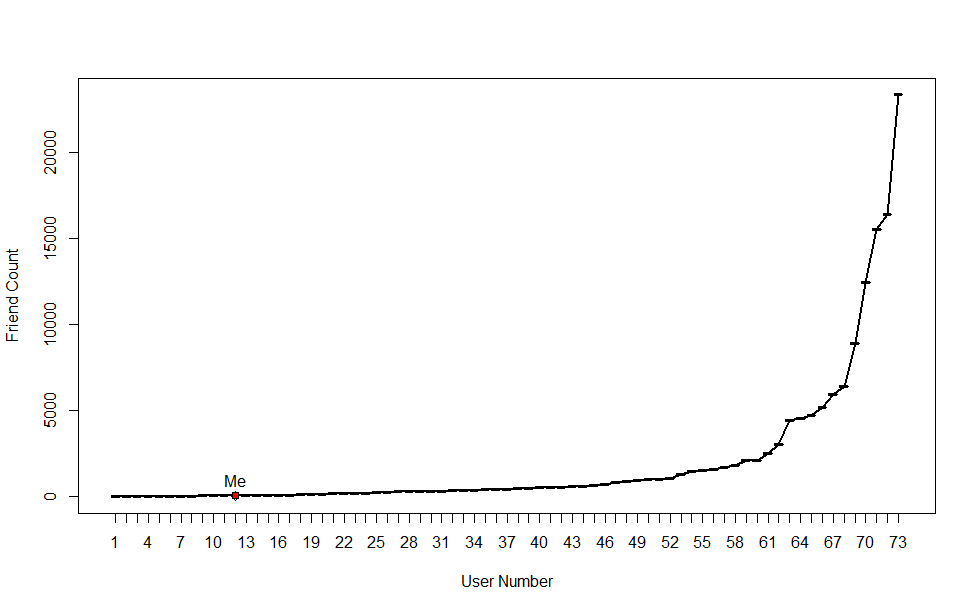
\includegraphics[width=1\textwidth]{twitter}
\caption{Twitter Number of Friends per Friend}
\label{fig:twitter}
\end{figure}

\subsection{Python Code}
%%% Code Listing%%%%%

\lstset{
    language=python,
    caption={Twitter Friend Counts},
     label=code:tcount
}

\lstinputlisting{twitter_friends.py}

\lstset{
    language=python,
    caption={Calculations},
     label=code:calc
}

\lstinputlisting{calculate.py}
\newpage 
%----------------------------------------------------------------------------------------
%           TASK 2
%----------------------------------------------------------------------------------------

\section{Facebook Friends}
Using your facebook account, repeat question \#1 (if you have >
50 friends).

\subsection{Solution}

I was able to extract my Facebook friends' friends using the code, ``seleniumScrapePB.py'',  provided by classmate Alexander Nwala. 
Firefox is required to use it and gave me an error because I was working on a Centos server without a display.
I used Xvfb to create an ``X server that doesn't require connection to a physical display.''\cite{bib:firefox}
A Python program was written to parse and sort the resulting CSV file, ``facebookFriendFriendsCountTuples.txt.'' \cite{bib:csv}
I added myself to the list and wrote the result to a file to be used to create the friendship graph.
The output file ``facebook.txt'' is included with this report.
Additionally, the mean, median, and standard deviation were computed using the same calculate program used for Twitter.
The result of the calculations was appended to the same file with the Twitter calculations.
Several of my friends and family members have over a thousand Facebook friends, which accounts for the high standard deviation.
I calculated that I am in the tenth percentile, which is well below the average and median.
Listing \ref{code:fb} is the python program used to convert the csv into the tabular, sorted text file and perform the calculations.
Table \ref{table:fb-calc} shows the calculation results for Facebook.

\begin{table}[H]
\centering
\begin{tabular}{|l|l|l|l|l|l|}
\hline
Mean & 484.42 \\
\hline
Median &  290 \\
\hline
Std. Dev & 697.54 \\
\hline
\end{tabular}
\caption{Facebook Statistics}
\label{table:fb-calc}
\end{table}

R was used to create the graph from the output file.
A large dot was placed on the graph with the text ``Me'' to denote my position on it, shown in Figure \ref{fig:facebook}.\cite{bib:rline}
I am at position 9 of 95, so most of my friends have more friends than I do.  
The majority of my friends with fewer number of friends are older family members whose only friends are other family members, so it makes sense.
The code used to create the graph is also in file ``a5.r'', included in this report.

\begin{figure}[H]
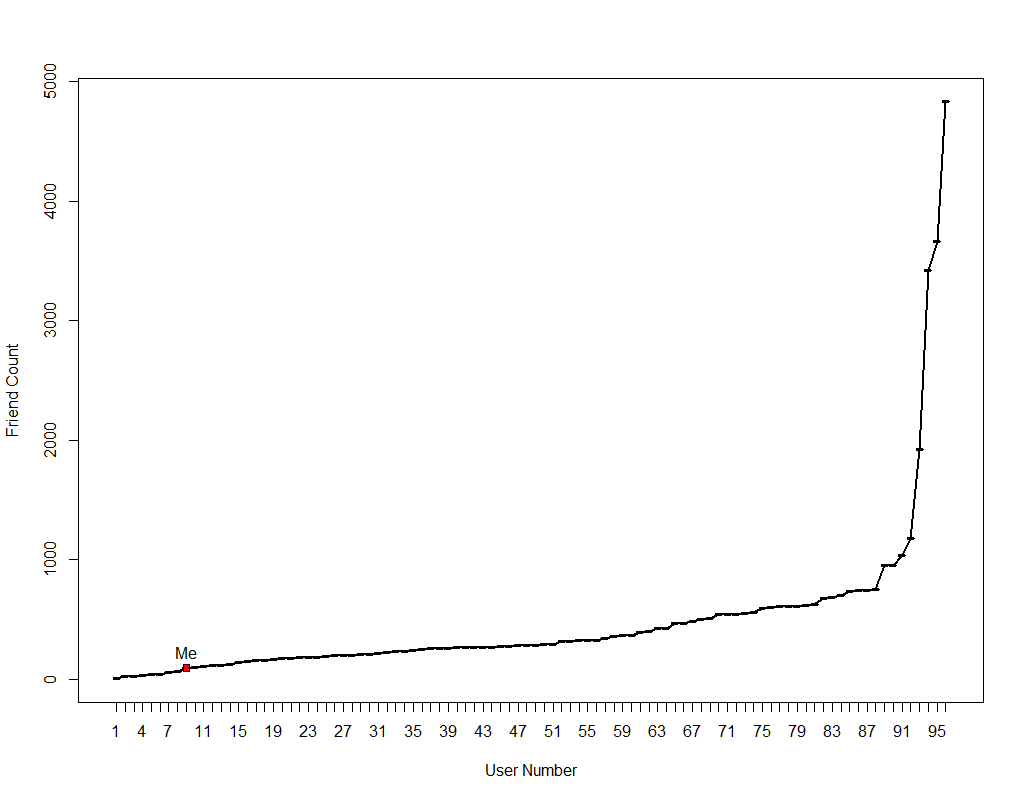
\includegraphics[width=1\textwidth]{facebook-graph}
\caption{Facebook Number of Friends per Friend}
\label{fig:facebook}
\end{figure}

\newpage
\subsection{Python Code}
%%% Code Listing%%%%%
\lstset{
    language=python,
    caption={Convert Output},
     label=code:fb
}

\lstinputlisting{convertcsv.py}
\newpage
%----------------------------------------------------------------------------------------
%            TASK 3
%----------------------------------------------------------------------------------------

\section{Linkedin Connections}
Using your linkedin account, repeat question \#1 (if you have >
50 connections).

\subsection{Solution}

 There are caveats to the Linkedin Connections API.
It is easy to retrieve your own connection numbers, but a first-degree connection must have a third-party accessible profile.
Additionally, Linkedin puts a cap on the number of connections reported.
If a person has more then 500 connections, 500 is the number given.\cite{bib:l-profile}
I found that I had only 39 connections and 34 do not have a private profile.
Five connections were retrieved with 500, so they have 500 or more.
Although this is under the 50 requirement, I still wanted to see if it followed the friendship paradox.
Only four of my connections have fewer connections, and two of those four are recent college graduates.
This puts me in the thirteenth percentile.
The mean, median, and standard deviation were computed again and the result was appended to the same file with the Twitter and Facebook calculations.
Listing \ref{code:li} is the python program connect to the Linkedin API, create the sorted text file, and perform the calculations. \cite{bib:py-linkedin}
Listing \ref{code:lio} is the python program used to set up the initial Oauth with the API.\cite{bib:l-oauth}
Table \ref{table:li-calc} shows the statistics results for Linkedin.

\begin{table}[H]
\centering
\begin{tabular}{|l|l|l|l|l|l|}
\hline
Mean &  211.55\\
\hline
Median &  175 \\
\hline
Std. Dev &  157\\
\hline
\end{tabular}
\caption{Linkedin Statistics}
\label{table:li-calc}
\end{table}

R was used to create the graph from the output file.
A large dot was placed on the graph with the text ``Me'' to denote my position on it, shown in Figure \ref{fig:linkedin}.\cite{bib:rline}
I am at position 5 of 39, so as expected, most of my connections have more connections than I do.  
The code used to create the graph was also added to file ``a5.r,'' which is included in this report.

\begin{figure}[H]
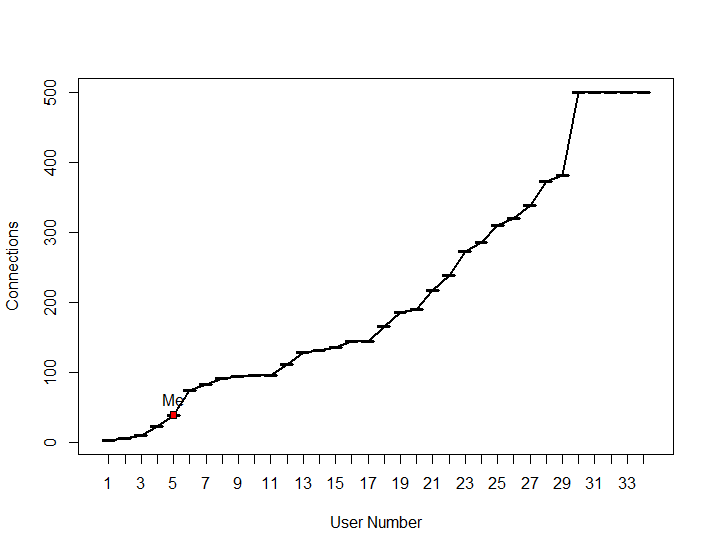
\includegraphics[width=1\textwidth]{linkedin-conn}
\caption{Linkedin Number of Friends per Friend}
\label{fig:linkedin}
\end{figure}

\subsection{Python Code}
%%% Code Listing%%%%%
\lstset{
    language=python,
    caption={Linkedin Connections},
     label=code:li
}

\lstinputlisting{linkedin_connections.py}

\lstset{
    language=python,
    caption={Linkedin Oauth},
     label=code:lio
}

\lstinputlisting{linkedin_oath.py}
\newpage

\bibliography{references}{}
\bibliographystyle{plain}
\end{document}